%%%%%%%%%%%%%%%%%%%%%%%%%%%%%%%%%%%%%%%%%%%%%%%%%%%%%%%%%%%%%%%%%%%%%%%%%%%%%%%%
% TUM-Vorlage: Präsentation
%%%%%%%%%%%%%%%%%%%%%%%%%%%%%%%%%%%%%%%%%%%%%%%%%%%%%%%%%%%%%%%%%%%%%%%%%%%%%%%%
%
% Rechteinhaber:
%     Technische Universität München
%     https://www.tum.de
%
% Gestaltung:
%     ediundsepp Gestaltungsgesellschaft, München
%     http://www.ediundsepp.de
%
% Technische Umsetzung:
%     eWorks GmbH, Frankfurt am Main
%     http://www.eworks.de
%
%%%%%%%%%%%%%%%%%%%%%%%%%%%%%%%%%%%%%%%%%%%%%%%%%%%%%%%%%%%%%%%%%%%%%%%%%%%%%%%%


%%%%%%%%%%%%%%%%%%%%%%%%%%%%%%%%%%%%%%%%%%%%%%%%%%%%%%%%%%%%%%%%%%%%%%%%%%%%%%%%
% Zur Wahl des Seitenverhältnisses bitte einen der beiden folgenden Befehle
% auskommentieren und den ausführen lassen:
%\documentclass[aspectratio=169]{beamer}
\documentclass[notes,t,aspectratio=169]{beamer}
\usepackage[
    orientation=landscape,
    size=custom,
    width=25.4,
    height=14.2875,
    scale=0.5
]{beamerposter}

% Display Notes for pympress
\usepackage{pgfpages}
\setbeameroption{show notes on second screen=right}
\setbeamertemplate{note page}[plain]
\setbeamerfont{note page}{size=\Large}

\newcommand{\PraesentationSchriftgroesseSehrGross}{\fontsize{25}{38}}
\newcommand{\PraesentationSchriftgroesseGross}{\fontsize{18}{27}}
\newcommand{\PraesentationSchriftgroesseNormal}{\fontsize{14}{21}}
\newcommand{\PraesentationSchriftgroesseKlein}{\fontsize{11}{17}}
\newcommand{\PraesentationSchriftgroesseDreizeiler}{\fontsize{7}{10}}
\newcommand{\PraesentationSchriftgroesseAufzaehlungszeichen}{\fontsize{10}{8}}

\newcommand{\PraesentationAbstandAbsatz}{18pt}
\newcommand{\PraesentationPositionKorrekturOben}{-1cm}
\newcommand{\PraesentationBeispieleSchriftgroessen}{25 | 18 | 14 | 11}
\usepackage[utf8]{inputenc}
\usepackage[T1]{fontenc} % Zeichensatzkodierung

\usepackage{calc} % Berechnungen

\usepackage[ngerman]{babel} % Deutsche Lokalisierung
\usepackage{graphicx} % Grafiken
\usepackage[absolute, overlay]{textpos} % Positionierung

% Silbentrennung:
\usepackage{hyphenat}
%\tolerance 2414
%\hbadness 2414
%\emergencystretch 1.5em
%\hfuzz 0.3pt
%\widowpenalty=10000     % Hurenkinder
%\clubpenalty=10000      % Schusterjungen
%\vfuzz \hfuzz

% Euro-Symbol:
\usepackage[gen]{eurosym}
\DeclareUnicodeCharacter{20AC}{\euro{}}

% Schriftart Helvetica:
\usepackage[scaled]{helvet}
\renewcommand{\familydefault}{\sfdefault}

\usepackage{mathptmx} % skalierbare Formelschriften

\usepackage{tabularx}

\usepackage{multicol} % mehrspaltiger Text

\usepackage{tikz}
\usetikzlibrary{arrows, shapes, shapes.multipart, trees, positioning,
    backgrounds, fit, matrix, external, overlay-beamer-styles}

% Diagramme:
\usepackage{pgfplots}
\pgfplotsset{compat=default}

% Erweiterbare Fusszeile:
\newcommand{\PraesentationFusszeileZusatz}{}

\usepackage{bookmark} % Lesezeichen

% Unterdrückung layoutbedingter Warnungen
\usepackage[immediate]{silence}
\WarningFilter[layout]{lastpage}{Rerun to get the references right} % Gesamtseitenzahl
\WarningFilter[layout]{latex}{Label(s) may have changed.} % Referenz auf letzte Seite
\WarningFilter[layout]{pgfplots}{running in backwards compatibility mode (unsuitable tick labels; missing features).} % Labelerstellung ab Version 1.17 nicht abwärtskompatibel
\WarningFilter[layout]{latex}{There were undefined references}
\WarningFilter[layout]{latex}{Reference `PraesentationDiagramm} % Erstellung einer Legende außerhalb des Diagrammbereichs

% Debugging:
%\DeactivateWarningFilters[layout] % Unterdrückte Warnungen einschalten
\usepackage{listings}

\lstdefinelanguage{rv64}{
    morekeywords={
        addi, bne,
        a1, x0
    },
    sensitive=false
}

\definecolor{SbtComment}{RGB}{80, 80, 80}

\lstdefinelanguage{SbtIr}{
    morekeywords={
        block,
        i64, i32, i16, i8, imm,
        immediate, add,
        cjump, jump
    },
    morecomment=[l]{//},
    morecomment=[s]{/*}{*/}
}

\usepackage[verbatim]{lstfiracode}
\lstset{
    style=FiraCodeStyle, % Use predefined FiraCodeStyle
    basicstyle=\ttfamily, % Use \ttfamily for source code listings
    keywordstyle=\color{TUMBlauDunkel},
    commentstyle=\color{SbtComment}
}

 % Seitenverhältnis 16:9
%%%%%%%%%%%%%%%%%%%%%%%%%%%%%%%%%%%%%%%%%%%%%%%%%%%%%%%%%%%%%%%%%%%%%%%%%%%%%%%%


%%%%%%%%%%%%%%%%%%%%%%%%%%%%%%%%%%%%%%%%%%%%%%%%%%%%%%%%%%%%%%%%%%%%%%%%%%%%%%%%
%%%%%%%%%%%%%%%%%%%%%%%%%%%%%%%%%%%%%%%%%%%%%%%%%%%%%%%%%%%%%%%%%%%%%%%%%%%%%%%%
% TUM-Vorlage: Personenspezifische Informationen
%%%%%%%%%%%%%%%%%%%%%%%%%%%%%%%%%%%%%%%%%%%%%%%%%%%%%%%%%%%%%%%%%%%%%%%%%%%%%%%%
%
% Rechteinhaber:
%     Technische Universität München
%     https://www.tum.de
% 
% Gestaltung:
%     ediundsepp Gestaltungsgesellschaft, München
%     http://www.ediundsepp.de
% 
% Technische Umsetzung:
%     eWorks GmbH, Frankfurt am Main
%     http://www.eworks.de
%
%%%%%%%%%%%%%%%%%%%%%%%%%%%%%%%%%%%%%%%%%%%%%%%%%%%%%%%%%%%%%%%%%%%%%%%%%%%%%%%%

% Für die Person anpassen:

% Allgemein:
\newcommand{\AllgemeinGestalter}{ediundsepp Gestaltungsgesellschaft}
\newcommand{\AllgemeinErsteller}{eWorks GmbH}

% Universität:
\newcommand{\UniversitaetName}{Technische Universität München}
\newcommand{\UniversitaetAbkuerzung}{TUM}
\newcommand{\UniversitaetWebseite}{www.tum.de}
\newcommand{\UniversitaetLogoBreite}{19mm}
\newcommand{\UniversitaetLogoHoehe}{1cm}

\newcommand{\UniversitaetAdresse}{%
	Arcisstraße~21\\%
	80333~München%
}

\hyphenation{} % eigene Silbentrennung
                    % !!! DATEI ANPASSEN !!!
%%%%%%%%%%%%%%%%%%%%%%%%%%%%%%%%%%%%%%%%%%%%%%%%%%%%%%%%%%%%%%%%%%%%%%%%%%%%%%%%

\newcommand{\Datum}{\today}

\renewcommand{\PraesentationFusszeileZusatz}{Rechnerarchitektur-Großpraktikum 2021 | Statische Binärübersetzung von RISC-V in x86-64}

\title{Statische Binärübersetzung von RISC-V in x86-64}
\author{Lukas Döllerer, Jonathan Hettwer, Johannes Maier, Tobias Schwarz, Felix Solcher}
\institute[]{Rechnerarchitektur-Großpraktikum 2021}
\date[\Datum]{Garching, 16. Juli 2021}
\subject{Statische Binärübersetzung von RISC-V in x86-64}


%%%%%%%%%%%%%%%%%%%%%%%%%%%%%%%%%%%%%%%%%%%%%%%%%%%%%%%%%%%%%%%%%%%%%%%%%%%%%%%%
%%%%%%%%%%%%%%%%%%%%%%%%%%%%%%%%%%%%%%%%%%%%%%%%%%%%%%%%%%%%%%%%%%%%%%%%%%%%%%%%
% EINSTELLUNGEN
%%%%%%%%%%%%%%%%%%%%%%%%%%%%%%%%%%%%%%%%%%%%%%%%%%%%%%%%%%%%%%%%%%%%%%%%%%%%%%%%

\newcommand{\PraesentationSeitenrand}{8.9mm}
\newcommand\crule[3][black]{\textcolor{#1}{\rule{#2}{#3}}}

\newlength\smallerbaselineskip
\setlength{\smallerbaselineskip}{0.8\baselineskip}

    % Blautöne:
\definecolor{TUMBlau}{RGB}{0,101,189} % Pantone 300
\definecolor{TUMBlauDunkel}{RGB}{0,82,147} % Pantone 301
\definecolor{TUMBlauHell}{RGB}{152,198,234} % Pantone 283
\definecolor{TUMBlauMittel}{RGB}{100,160,200} % Pantone 542

    % Hervorhebung:
\definecolor{TUMElfenbein}{RGB}{218,215,203} % Pantone 7527 -Elfenbein
\definecolor{TUMGruen}{RGB}{162,173,0} % Pantone 383 - Grün
\definecolor{TUMOrange}{RGB}{227,114,34} % Pantone 158 - Orange
\definecolor{TUMGrau}{gray}{0.6} % Grau 60%


\setbeamercolor*{alerted text}{fg=TUMOrange}

\newcommand{\PraesentationSetzeTextfarbe}{
    \color{PraesentationTextfarbe}
    \setbeamercolor*{frametitle}{fg=PraesentationTextfarbe}
    \setbeamercolor*{normal text}{fg=PraesentationTextfarbe}
    \setbeamercolor{itemize/enumerate body}{fg=PraesentationTextfarbe}
    \setbeamercolor*{itemize item}{fg=PraesentationTextfarbe}
}

\newcommand{\PraesentationFarbschemaStandard}{
    \setbeamercolor*{background canvas}{}
    \definecolor{PraesentationTextfarbe}{rgb}{0,0,0}
    \PraesentationSetzeTextfarbe
}

\newcommand{\PraesentationFarbschemaWeissBlau}{
    \setbeamercolor*{background canvas}{bg=TUMBlauDunkel}
    \definecolor{PraesentationTextfarbe}{rgb}{1,1,1}
    \PraesentationSetzeTextfarbe
}

\newcommand{\PraesentationFarbschemaWeissSchwarz}{
    \setbeamercolor*{background canvas}{bg=black}
    \definecolor{PraesentationTextfarbe}{rgb}{1,1,1}
    \PraesentationSetzeTextfarbe
}

\newcommand{\PraesentationTitelseiteInhalt}{
    \begin{textblock*}{\paperwidth}[0,0](0cm,-\PraesentationSeitenrand - 6.5mm + \PraesentationPositionKorrekturOben)%
        \color{PraesentationTextfarbe}%
        \frametitle{\inserttitle}
        \vspace*{49.4mm}
        \usebeamerfont{author}\selectfont\insertauthor\\
	    \vspace*{2mm}
        \insertinstitute\\
        \insertdate%
    \end{textblock*}
}

\newcommand{\PraesentationSeitenkopfInhalt}[1]{
    %\vspace*{31.7mm}%
    \begin{textblock*}{1.68cm}[1,0](\paperwidth - \PraesentationSeitenrand - \PraesentationSeitenrand, 0cm)%
        \includegraphics[width=1.68cm]{#1}%
    \end{textblock*}
    \begin{textblock*}{3cm}[1,0](\paperwidth - \PraesentationSeitenrand, -\PraesentationSeitenrand)%
        \hbox{%
            \color{PraesentationTextfarbe}
            \hbox{\insertframenavigationsymbol}%
            \hbox{\insertsubsectionnavigationsymbol}%
            \hbox{\insertsectionnavigationsymbol}%
        }%
    \end{textblock*}%
}

\newcommand{\PraesentationBildUhrenturm}{%
    \begin{textblock*}{10.82cm}[1,1](\paperwidth - \PraesentationSeitenrand - \PraesentationSeitenrand, \paperheight - 9mm)%
        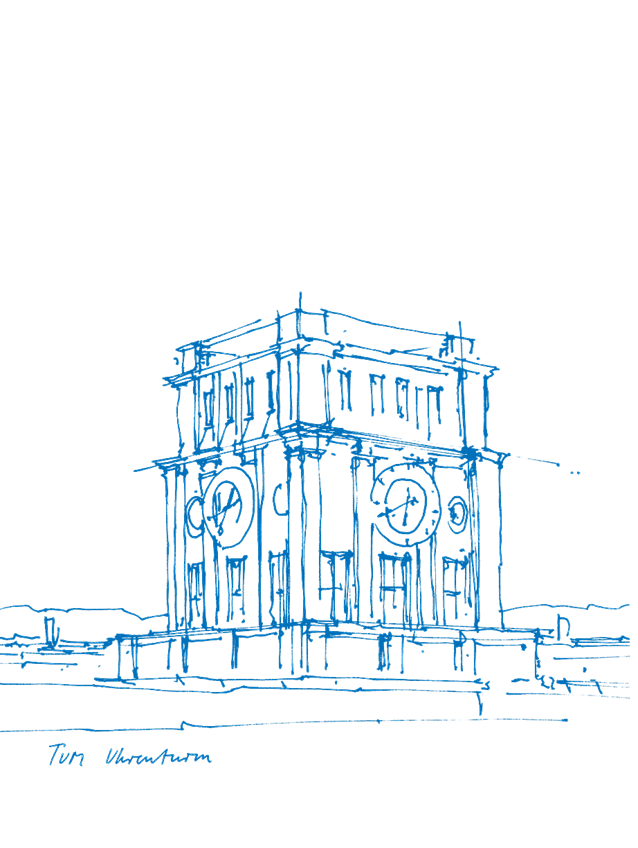
\includegraphics{img/TUM_Uhrenturm.png}%
    \end{textblock*}%
}

\newcommand{\PraesentationStartseiteUhrenturm}{
    \setbeamertemplate{title page}{%
        \PraesentationSeitenkopfInhalt{img/Universitaet_Logo_RGB.pdf}
        \PraesentationBildUhrenturm
        \PraesentationTitelseiteInhalt
    }
}

\newcommand{\PraesentationStartseiteLeer}{
    \setbeamertemplate{title page}{%
        \PraesentationSeitenkopfInhalt{img/Universitaet_Logo_weiss.pdf}
        \PraesentationTitelseiteInhalt
    }
}


\newcommand{\PraesentationMasterStandard}{
    \PraesentationFarbschemaStandard

    \PraesentationStartseiteUhrenturm

    \setbeamertemplate{headline}{
        \PraesentationSeitenkopfInhalt{img/Universitaet_Logo_RGB.pdf}
    }
}

\newcommand{\PraesentationMasterWeissBlau}{
    \PraesentationFarbschemaWeissBlau

    \PraesentationStartseiteLeer

    \setbeamertemplate{headline}{
        \PraesentationSeitenkopfInhalt{img/Universitaet_Logo_weiss.pdf}
    }
}

\newcommand{\PraesentationMasterKopfzeileDreizeiler}{
    \PraesentationFarbschemaStandard

    \setbeamertemplate{title page}{%
        \PraesentationBildUhrenturm
        \begin{textblock*}{\paperwidth}[0,0](0cm, -7.8mm)%
            \color{TUMBlau}\PraesentationSchriftgroesseDreizeiler\selectfont%
            \LehrstuhlName\\%
            \FakultaetName\\%
            \UniversitaetName\\%
            \normalcolor\normalsize\selectfont%
        \end{textblock*}%
        \PraesentationSeitenkopfInhalt{img/Universitaet_Logo_RGB.pdf}
        \PraesentationTitelseiteInhalt
    }

    \setbeamertemplate{headline}{
        \begin{textblock*}{\paperwidth}[0,0](0cm, -7.8mm)%
            \color{TUMBlau}\PraesentationSchriftgroesseDreizeiler\selectfont%
            \LehrstuhlName\\%
            \FakultaetName\\%
            \UniversitaetName\\%
            \normalcolor\normalsize\selectfont%
        \end{textblock*}%
        \PraesentationSeitenkopfInhalt{img/Universitaet_Logo_RGB.pdf}
    }
}

\newcommand{\PraesentationMasterWeissSchwarz}{
    \PraesentationFarbschemaWeissSchwarz

    \setbeamertemplate{title page}{%
        \PraesentationTitelseiteInhalt
        \PraesentationSeitenkopfInhalt{img/Universitaet_Logo_weiss.pdf}
    }

    \setbeamertemplate{headline}{
        \PraesentationSeitenkopfInhalt{img/Universitaet_Logo_weiss.pdf}
    }
}

\newcommand{\PraesentationTitelseite}{\frame[plain]{\titlepage}}
\newcommand{\PraesentationUeberschriftZweizeilig}[2]{\frametitle{#1\\[8mm]#2}}

\setbeamersize{
    text margin left=\PraesentationSeitenrand,
    text margin right=\PraesentationSeitenrand
}

\setbeamertemplate{frametitle}{%
    {\rule{0pt}{42mm + \PraesentationPositionKorrekturOben}\PraesentationSchriftgroesseSehrGross\selectfont\insertframetitle\newline\vspace*{-6.7mm}}%
}

% Aufzählungen:
\newcommand{\PraesentationAufzaehlungEbeneEinsSymbol}{\raise2pt\hbox{\donotcoloroutermaths\usebeamercolor{itemize subitem}\PraesentationSchriftgroesseAufzaehlungszeichen$\bullet$}}
\newcommand{\PraesentationAufzaehlungEbeneZweiSymbol}{\raise1.25pt\hbox{\donotcoloroutermaths\usebeamercolor{itemize subitem}$-$}}
\setbeamertemplate{itemize items}[circle]
\setbeamertemplate{itemize subitem}[triangle]
\setbeamercolor{itemize subitem}{fg=black}
\setbeamerfont{itemize/enumerate subbody}{size=\normalsize}
\setbeamertemplate{itemize item}{\PraesentationAufzaehlungEbeneEinsSymbol}
\setbeamertemplate{itemize subitem}{\PraesentationAufzaehlungEbeneZweiSymbol{}}
%\addtolength{\leftmarginii}{16mm-2pt}%

\newenvironment{PraesentationAufzaehlung}
{%
    \vspace{-\baselineskip}%
    \begin{itemize}%
        \setlength{\itemsep}{0pt}%
        \setlength{\parskip}{0pt}%
        \setlength{\parsep}{0pt}%
        \addtolength{\itemindent}{-1ex}%
}{%
    \end{itemize}%
}

%%%%%%%%%%%%%%%%%%%%%%%%%%%%%%%%%%%%%%%%%%%%%%%%%%%%%%%%%%%%%%%%%%%%%%%%%%%%%%%%
% DOKUMENT
%%%%%%%%%%%%%%%%%%%%%%%%%%%%%%%%%%%%%%%%%%%%%%%%%%%%%%%%%%%%%%%%%%%%%%%%%%%%%%%%


% PDF-Einstellungen:
\hypersetup{
    pdfstartview={Fit},
    pdfproducer={\AllgemeinErsteller},
    pdfcreator={\AllgemeinGestalter}
}

\textblockorigin{\PraesentationSeitenrand}{\PraesentationSeitenrand} % Ursprung für Positionierung

\setbeamerfont{footnote}{size=\PraesentationSchriftgroesseKlein}

\setbeamertemplate{footline}{
    \hbox{%
        \usebeamerfont{footnote}%
        \begin{beamercolorbox}[wd=.9\paperwidth]{}%
            \hspace*{\PraesentationSeitenrand}%
            \PraesentationFusszeileZusatz{}%
        \end{beamercolorbox}%
        \begin{beamercolorbox}[wd=.1\paperwidth]{}%
            \insertframenumber{}%
            \raggedleft
            \hspace*{\PraesentationSeitenrand}%
        \end{beamercolorbox}%
        \vspace*{3.25mm}%
    }%
}

\setbeamertemplate{navigation symbols}{}

\begin{document}
\setlength{\baselineskip}{\PraesentationAbstandAbsatz}
\setlength{\parskip}{\baselineskip}
 % !!! NICHT ENTFERNEN !!!
%%%%%%%%%%%%%%%%%%%%%%%%%%%%%%%%%%%%%%%%%%%%%%%%%%%%%%%%%%%%%%%%%%%%%%%%%%%%%%%%


%%%%%%%%%%%%%%%%%%%%%%%%%%%%%%%%%%%%%%%%%%%%%%%%%%%%%%%%%%%%%%%%%%%%%%%%%%%%%%%%
% FOLIENSTIL: Standard
\PraesentationMasterStandard

\PraesentationTitelseite % Fügt die Startseite ein


% draws an arrow from (#2,#3) to (#2+#4,#3) with height of #5 (arrow in x direction)
% color (and other arguments, like visible on), startX, startY, length (X dir), height (Y dir)
\newcommand{\TikZArrowX}[5]{
    \filldraw[#1] (#2,#3) -- (#2,#3+#5*2/3) -- (#2+#4/2,#3+#5*2/3) -- (#2+#4/2,#3+#5) -- (#2+#4,#3) -- (#2+#4/2,#3-#5) -- (#2+#4/2,#3-#5*2/3) -- (#2,#3-#5*2/3) -- (#2,#3);
    \draw[#1, black] (#2,#3) -- (#2,#3+#5*2/3) -- (#2+#4/2,#3+#5*2/3) -- (#2+#4/2,#3+#5) -- (#2+#4,#3) -- (#2+#4/2,#3-#5) -- (#2+#4/2,#3-#5*2/3) -- (#2,#3-#5*2/3) -- (#2,#3);
}

% draws an arrow from #2,#3) to (#2,#3+#5) with height of #4 (arrow in y direction)
% color (and other arguments, like visible on), startX, startY, length (X dir), height (Y dir), color
\newcommand{\TikZArrowY}[5]{
    \filldraw[#1] (#2,#3) -- (#2+#4*2/3,#3) -- (#2+#4*2/3,#3+#5/2) -- (#2+#4,#3+#5/2) -- (#2,#3+#5) -- (#2-#4,#3+#5/2) -- (#2-#4*2/3,#3+#5/2) -- (#2-#4*2/3,#3) -- (#2,#3);
    \draw[#1, black] (#2,#3) -- (#2+#4*2/3,#3) -- (#2+#4*2/3,#3+#5/2) -- (#2+#4,#3+#5/2) -- (#2,#3+#5) -- (#2-#4,#3+#5/2) -- (#2-#4*2/3,#3+#5/2) -- (#2-#4*2/3,#3) -- (#2,#3);
}

% draws one entry of the color legend for the program scheme
% color, text, posX, posY (left, top coordinate)
\newcommand{\colorLegendEntry}[4]{
    \filldraw[#1] (#3,#4) rectangle (#3+1,#4+1);
    \draw[black] (#3,#4) rectangle (#3+1,#4+1);
    \node at (#3+0.5,#4+0.4) (color_legend_entry_point) {};
    \node[right=2mm of color_legend_entry_point] (color_legend_entry_text) {#2};
}

% draws a color legend for the program scheme
% posX, posY (left, top coordinate)
\newcommand{\colorLegend}[2] {
    \colorLegendEntry{TUMOrange}{Static Translator Parts}{#1}{#2}
    \colorLegendEntry{TUMBlauDunkel}{Immediate Representation (IR)}{#1}{#2-1.5}
    \colorLegendEntry{purple}{Maschine Code / ELF File}{#1}{#2-3}
}

% draws the schematic presentation of the program
% scale, fontSize
\newcommand{\ProgramSchemeVersionOne}[2]{
    \begin{center}
        \begin{tikzpicture}[very thick, scale=#1]
            % draw color legend
            \colorLegend{-2}{-6}

            % riscv elf file rectangle
            % background
            \filldraw[purple] (-2,-2) rectangle (2,2);
            % black border
            \draw[black] (-2,-2) rectangle (2,2);
            % label
            \node[align=center, color=white] at (0,0) (riscv_text) {\fontsize{#2}{#2} \selectfont RISC-V};

            % lifter arrow
            \TikZArrowX{TUMOrange}{2}{0}{6}{1.5}
            % arrow label
            \node[align=center, color=white] at (4.5,0) (lifter_text) {\fontsize{#2}{#2} \selectfont Lifter};

            % ir (unoptimized) rectangle
            % background
            \filldraw[TUMBlauDunkel] (8,-2) rectangle (12,2);
            % black border
            \draw[black] (8,-2) rectangle (12,2);
            % label
            \node[align=center, color=white] at (10,0) (ir_text_1) {\fontsize{#2}{#2} \selectfont IR};

            % optimizer arrow
            \TikZArrowX{TUMOrange}{12}{0}{6}{1.5}
            % arrow label
            \node[align=center, color=white] at (14.5,0) (optimizer_text) {\fontsize{#2}{#2} \selectfont Optimizer};

            % ir (optimized) rectangle
            % background
            \filldraw[TUMBlauDunkel] (18,-2) rectangle (22,2);
            % black border
            \draw[black] (18,-2) rectangle (22, 2);
            % label
            \node[align=center, color=white] at (20,0) (ir_text_2) {\fontsize{#2}{#2} \selectfont IR};

            % compiler arrow
            \TikZArrowX{TUMOrange}{22}{0}{6}{1.5}
            % arrow label
            \node[align=center, color=white] at (24.5,0) (generator_text) {\fontsize{#2}{#2} \selectfont Generator};

            % x86_64 rectangle
            %background
            \filldraw[purple] (28,-2) rectangle (32,2);
            % black border
            \draw[black] (28,-2) rectangle (32,2);
            % label
            \node[align=center, color=white] at (30,0) (x86_64_text) {\fontsize{#2}{#2} \selectfont x86\_64};
        \end{tikzpicture}
    \end{center}
}



%%%%%%%%%%%%%%%%%%%%%%%
%% Programmübersicht %%
%%%%%%%%%%%%%%%%%%%%%%%

\begin{frame}
    \frametitle{Programmübersicht}
    \note[item]{Ziel: Statische Binärübersetzung}
    \note[item]{Übersetzung von Binärdateien auf eine andere Plattform}
    \note[item]{Dynamisch wäre ein Interpreter, also zur Laufzeit, bei uns Übersetzung zur Compilezeit}
    \note[item]{hier: von RISC-V zu x86\_64}
    \note[item]{RISC, feste 32-Bit Befehlslänge}
    \note[item]{wenige, einfache Befehle -> geringe Codedichte, aber leicht zu übersetzten}
    \note[item]{Register-Register-Maschine, also nur Operation auf Registern in der Dreioperandenform, s. 'ERA'}
    \note[item]{Lifter 'hebt' RISC-V in die Zwischenrepräsentation (sog. IR)}
    \note[item]{Optimierung auf der IR: aktuell noch Identitätsbbildung}
    \note[item]{Compiler compiliert zu Assemlby Code und dieser wird zu einer ausführbaren Datei assembliert}

    %alignment to have some space between headline an the schematic
    ~\\
    ~\\
    \ProgramSchemeVersionOne{0.6}{18}
\end{frame}

%%%%%%%%%%%%%%%%%%%%%
%% IR Aufbau Folie %%
%%%%%%%%%%%%%%%%%%%%%

\begin{frame}
    \frametitle{Intermediate Representation}{Aufbau}
    \note[item]{Selbst definierte Zwischenrepräsentation}
    \note[item]{Hauptbestandteil: Basic Blocks}
    \note[item]{-> Sequentielle Folge von Instruktionen, die durch Kontrollflussoperation beendet werden}
    \note[item]{Basic Block enthält Variablen in sogenannter SSA-Form und die dazu gehörenden Operationen}
    \note[item]{Static single assignment -> Jeder var wird nur einmal Wert zugewiesen}
    \note[item]{-> Vereinfacht Optimierungen}
    \note[item]{Eingaben kommen als "Statics" -> Abstrakte Darstellung von RISCV-Registern}
    \note[item]{Kontrollflussoperationen verbinden die Basic Blocks}
    \note[item]{SSA bedeutet: Variablen frei verschiebbar, deshalb Memory Tokens für Einhaltung der Reihenfolge}
    \pause{}
    \begin{itemize}
        \item Die IR besteht aus mehreren "`\textbf{Basic Blocks}"'
              \pause{}
        \item Basic Block: Eine Folge von sequentiellen Instruktionen, beendet durch eine Kontrollflussoperation
              \pause{}
        \item Ein Basic Block enthält Variablen in SSA-Form und dazugehörige Operationen
              \pause{}
        \item \textbf{Static single assignment (SSA):} Jeder Variable wird genau einmal ein Wert zugewiesen
              \pause{}
        \item Ein Basic Block erhält Eingaben in Form von Statics
              \pause{}
        \item Die Basic Blocks sind durch die Kontrollflussoperationen miteinander verbunden
              \pause{}
        \item Zur Nachvervolgung von Lese- und Schreiboperationen gibt es Memory Tokens $\rightarrow$ Optimierungen
    \end{itemize}
\end{frame}

\begin{frame}
    \frametitle{Intermediate Representation}{Operationen}
    \pause{}

    ~\\
    ~\\

    \begin{columns}[c]
        \column{0.4\textwidth}
        Instruktionen:
        \begin{itemize}
            \item Speicher: \texttt{store}, \texttt{load}
            \item Arithmetisch: \texttt{add}, \texttt{sub}, \texttt{mul}, ...
            \item Logisch: \texttt{and}, \texttt{or}, \texttt{shl}, ...
            \item Sonstige: Typkonvertierung, ...
        \end{itemize}

        \pause{}
        \column{0.4\textwidth}
        Kontrollflussoperationen:
        \begin{itemize}
            \item Sprünge: \texttt{jump}, \texttt{ijump}, \texttt{cjump}
            \item \texttt{unreachable}
            \item \texttt{syscall}
        \end{itemize}
    \end{columns}
\end{frame}

%%%%%%%%%%%%%%
%% IR Folie %%
%%%%%%%%%%%%%%

\begin{frame}[fragile]
    \frametitle{Intermediate Representation}{Beispiel}
    \pause{}
    ~\\
    ~\\
    ~\\
    \begin{columns}[c]
        \column{0.275 \textwidth}
        \begin{lstlisting}[language=rv64]
        [...]
        addi a0, x0, 100
        j somewhere_else
        [...]
        \end{lstlisting}

        \pause{}
        \column{0.125 \textwidth}
        \begin{tikzpicture}[scale=0.72]
            \TikZArrowX{TUMOrange}{0}{0}{4}{1}
        \end{tikzpicture}

        \pause{}

        \column{0.6 \textwidth}
        \begin{lstlisting}[language=SbtIr]
block b1(/* inputs */) <= [/* predecessors */] {
    i64 v0 <- @1
    [...] // more statics
    imm v32 <- immediate 0
    imm v33 <- immediate 100
    i64 v34 <- add imm v32, imm v33
} => [(jump, [b2, i64 v34])]
    \end{lstlisting}
    \end{columns}

\end{frame}
\clearpage

%%%%%%%%%%%%%%%%%%%%%%%%%%%
%% ELF File Parser Folie %%
%%%%%%%%%%%%%%%%%%%%%%%%%%%

\begin{frame}[fragile]
    \frametitle{Lifter}{ELF Binärdatei laden und Instruktionsbytes decodieren}
    \begin{columns}[c]
        \pause{}
        \column{0.5 \textwidth}
        \begin{enumerate}
            \note[item]{ELF Prüfung: Prüfbits, System-V ABI, 64-Bit, Little Endian, RISC-V Machine}
            \item ELF File prüfen.
            \note[item]{Symbole weren bei gestrippten ELF-Binaries nicht eingelesen}
            \item Program Header, Sections und Symbole auslesen.
            \note[item]{32-Byte bzw. 16-Byte Compressed mit frvdec decodieren}
            \item Section Bytes $\rightarrow$ Instruktionen durch \textbf{frvdec} decodieren.
        \end{enumerate}
        \column{0.50 \textwidth}
        \begin{lstlisting}[basicstyle=\footnotesize, breaklines=true, escapeinside={@@}]
ELF Header:
    Magic:   7f 45 4c 46 02 01 01 00 00 00 00 00 00 00 00 00
    Class:                             @\textcolor{TUMBlauDunkel}{ELF64}@
    Data:                              @\textcolor{TUMBlauDunkel}{2's complement, little endian}@
    Version:                           1 (current)
    OS/ABI:                            UNIX - @\textcolor{TUMBlauDunkel}{System V}@
    ABI Version:                       0
    Type:                              @\textcolor{TUMBlauDunkel}{EXEC}@ (Executable file)
    Machine:                           @\textcolor{TUMBlauDunkel}{RISC-V}@
    Version:                           0x1
    Entry point address:               @\textcolor{TUMBlauDunkel}{0x100b0}@
    Start of program headers:          64 (bytes into file)
    Start of section headers:          688 (bytes into file)
    Flags:                             0x5, RVC, double-float ABI
    Size of this header:               64 (bytes)
    Size of program headers:           56 (bytes)
    Number of program headers:         2
    Size of section headers:           64 (bytes)
    Number of section headers:         6
    Section header string table index: 5
        \end{lstlisting}
    \end{columns}
\end{frame}
\clearpage

%%%%%%%%%%%%%%%%%%%%%%%%%%
%% Lifter General Folie %%
%%%%%%%%%%%%%%%%%%%%%%%%%%

\begin{frame}
    \frametitle{Lifter}{RISC-V Instruktionen in IR Code umwandeln}
    \begin{enumerate}
        \pause{}
        \setlength\itemsep{0.6em}
        \item Instruktionen sequenziell lesen:
              \vspace{0.5em}
              \begin{enumerate}
                  \setlength\itemsep{0.6em}
                  \item Instruktionen in IR parsen
                  \item Wiederhole bis eine \textbf{Kontrollfluss ändernde Instruktion} auftritt
                  \item Beende Basic Block $\rightarrow$ starte neuen Basic Blöck für jede Kontrollflussänderung
                  \item Starte für jeden \textbf{neuen} Basic Block wieder bei 1
              \end{enumerate}
        \item Sollte Schritt 1 nicht alle vorhandenen Instruktionen in Basic Blöcke gepackt haben:\\ Beginne ab erster \textbf{unbetrachteter} Adresse / Instruktion erneut mit Schritt 1
    \end{enumerate}
\end{frame}
\clearpage

%%%%%%%%%%%%%%%%%%%%%%%%%%%%%%%%%%%%%%%
%% Lifter Backtracking und Splitting %%
%%%%%%%%%%%%%%%%%%%%%%%%%%%%%%%%%%%%%%%

\begin{frame}
    \frametitle{Lifter}{Lifter Splitting und Backtracking}
    \vspace{2em}
    \pause{}
    \begin{columns}[c]
        \column{0.4 \textwidth}
        \textbf{Aufteilen eines Basic Blocks}
        \note[item]{Sprung zurück in bereits geparsten Codebereich}
        \note[item]{Split an Einsprungaddresse und Verbindung mit direktem Sprung}
        \begin{itemize}
            \item Situation: Sprung \textbf{in} einen Basic Block
            \item Aufteilung an Sprungadresse in zwei Basic Blöcke
            \item Verbindung mit einem direkten Sprung
        \end{itemize}
        \pause{}
        \column{0.4 \textwidth}
        \textbf{Backtracking einer indirekten Sprungadresse}
        \note[item]{Indirekte Sprünge, also Sprünge mit Register als Eingabeparameter}
        \note[item]{Rekursives Backtracking um Wert des Registers zu ermitteln}
        \note[item]{Mehrere Werte möglich -> im Moment wird erster gewählt (mögliche Fehlerquelle)}
        \begin{itemize}
            \item rekursive Rückverfolgung aller Argumente
            \item für "`statics"' werden alle möglichen Vorgänger betrachtet
            \item Aussortierung von Vorgängern
        \end{itemize}
    \end{columns}
\end{frame}
\clearpage

\note[itemize]{
    \item {Ein Basic Block muss aufgeteilt werden, wenn eine Kontrollflussoperation an eine Adresse springt, welche bereits geliftet ist und sich in diesem Basic Block befindet}
    \item {Warum muss ein Basic Block geteilt werden? -> damit nach Definition der IR immer an den Beginn eines Basic Blocks gesprungen werden kann}
    \item {bei Schleifen nötig -> siehe IR Beispiel vorher}
    \item {Unbedingter Sprung als Verbindung (nach )}
    \item {Variablen anhand Zuweisungsadresse (Adresse der Instruktion, welche sie erzeugt hat) auf die beiden Basic Blöcke aufgeteilt}
    \item {Sorgt für Probleme, weil Datenstruktur verändert wird, v.a. richtige Aufteilen der Variablen, korrekter Sprung, korrekter Transfer der Cfops}
    \item {Die Kontrollflussoperationen werden in den zweiten Basic Block (mit der höheren Adresse) geschoben, weil diese das Ende des Basic Blocks sind und sich damit garantiert im zweiten Befinden}
}

%%%%%%%%%%%%%%%%%%%%%
%% Generator Folie %%
%%%%%%%%%%%%%%%%%%%%%

\begin{frame}
    \note[item]{Sehr einfache, aber korrekte Übersetztung}
    \note[item]{Originales ELF-Programm als binäres Speicherbild an exakter Adresse eingebunden}
    \note[item]{RISC-V System-V ABI (Startup, Syscall) zur Laufzeit emuliert}
    \note[item]{Stack wird nur initialisiert, danach nicht mehr im Generator speziell behandelt}
    \note[item]{Indirekte Sprünge werden per Lookup zur Laufzeit aufgelöst}
    \note[item]{Erste Optimierung: Eliminierung von Redundanzen bei den Statics}

    \frametitle{Generator}{Übersetztung der IR zu x86\_64}
    \pause
    \begin{itemize}
        \item Sehr einfache, aber korrekte Übersetztung
        \item Originales ELF-Programm als binäres Speicherbild an exakter Adresse eingebunden
              %        \item Stellt nur initialen Stack zur Verfügung % es wird nicht der x86-64 Stack verwendet
        \item RISC-V System-V ABI (Startup, Syscall) zur Laufzeit emuliert
        \item Indirekte Sprünge werden per Lookup zur Laufzeit aufgelöst
        \item Erste Optimierung: Eliminierung von Redundanzen bei den Statics
    \end{itemize}
\end{frame}
\clearpage

%%%%%%%%%%%%%%%%%%%%%%%%%%%%%%
%% Technische Demonstration %%
%%%%%%%%%%%%%%%%%%%%%%%%%%%%%%

\begin{frame}[fragile]
    \frametitle{Technische Demonstration}{Live Demonstration des aktuellen Standes}

    % Dauer: ~3m
    \note[item]{Kompilieren zu RISCV-64 mit einer unmodifizierten musl libc (standardbibliothek)}
    \note[item]{Unser Program übersetzt zu x86 assembly + binary image}
    \note[item]{Assemblieren mittels GNU tools}
    \note[item]{Linken von binary image, übersetztem assembly und hilfsbibliothek}
    \note[item]{Ausführen}
    \note[item]{Ausführen, ungefährere Vergleich (native, qemu, translated) => Wo sind wir mit optimierungen, fast faktor 10 langsamer als QEMU}

    % Setup:
    % Use xfc4, configure beamer as display to the right
    % Go To Workspace 1, start pympress with
    % LC_ALL=de_DE.UTF-8 pympress presentation/build/presentation_16_9.pdf
    % Go To Workspace 2, on laptop start xfce4-terminal with
    % 1. Open new Terminal Window on laptop with `tmux new-session -s demo -A`
    % 2. Open new Terminal Window on presentation screen with `tmux attach-session -r -t demo`
    % Resize as necessary (ctrl + + or -)
    %
    % Commands:
    % ./big_tests/sysroot/bin/riscv64-linux-gnu-gcc -static examples/helloworld3.c -o examples/helloworld3
    %
    % ./build/src/translate --debug=true --print-ir=true --output-binary=examples/helloworld3.bin --output=examples/helloworld3_translated.s examples/helloworld3
    % gcc -c examples/helloworld3_translated.s -o examples/helloworld3_translated.o
    % ld -T src/generator/x86_64/helper/link.ld examples/helloworld3_translated.o build/src/generator/x86_64/helper/libhelper.a -o examples/helloworld3_translated
    %
    % ./examples/helloworld3_translated
    %
    % Additional:
    % gcc examples/helloworld3.c -o examples/helloworld3_native
    % time ./examples/helloworld3_native
    % time ./examples/helloworld3
    % time ./examples/helloworld3_translated

    \begin{lstlisting}[language=bash, basicstyle=\footnotesize\ttfamily, extendedchars=true,escapeinside={@@}]
        ./big_tests/sysroot/bin/riscv64-linux-gnu-gcc \
            -static \
            examples/helloworld3.c \
            -o examples/helloworld3

        ./build/src/translate \
            @-@-debug=true \
            @-@-output-binary=examples/helloworld3.bin \
            @-@-output=examples/helloworld3_translated.s \
            examples/helloworld3

        gcc \
            -c examples/helloworld3_translated.s \
            -o examples/helloworld3_translated.o

        ld \
            -T src/generator/x86_64/helper/link.ld \
            examples/helloworld3_translated.o \
            build/src/generator/x86_64/helper/libhelper.a \
            -o examples/helloworld3_translated

        ./examples/helloworld3_translated
    \end{lstlisting}
\end{frame}
\clearpage

%%%%%%%%%%%%%%%%%%%%%
%% Erreichte Ziele %%
%%%%%%%%%%%%%%%%%%%%%

\begin{frame}
    \frametitle{Erreichte Ziele}{Erreichte Hauptziele und Ausblick}

    % Dauer: mind. 1 Minute, ansonsten flexible
    \note[item]{Freistehend => ohne standard bibliothek, z\.B\. handgeschriebenes assembly oder einfache C programme}
    \note[item]{Atomics werden nur also nicht atomics übersetzt so weit nötig}
    \note[item]{Demonstriert im Beispiel}
    \note[item]{2 Bugs in musl libc, malloc, fehlender BasicBlock in printf\_core wegen switch statement ohne control fluss änderung am ende von cases}
    \note[item]{Und noch vereinzelt weiter instructionen je nach bedarf}
    \note[item]{ijump eigentlich bei erweiterte Ziele, aber extrem wichtig da für return verwendet}

    \begin{itemize}
        \item Korrektes Übersetzen einfacher freistehender Programme
        \item Übersetzen von unmodifizierter musl libc
        \item Unterstützung von RV64I, RV64C, \ldots{}
        \item Auflösung indirekter Sprünge zur Laufzeit
    \end{itemize}
\end{frame}

%%%%%%%%%%%%%%%%%%%
%% Noch Fragen ? %%
%%%%%%%%%%%%%%%%%%%

\begin{frame}
    \frametitle{Noch Fragen?}{}
\end{frame}

%%%%%%%%%%%%%%%%%%%%%%%%%
%% Generator-Translate %%
%%%%%%%%%%%%%%%%%%%%%%%%%

\begin{frame}[fragile]
    \frametitle{Generator}
    \begin{columns}[c]
        \column{0.45 \textwidth}
        \begin{lstlisting}[language=SbtIr, escapechar=!]
        block b1(/* inputs */) <= [/* predecessors */] {
            !\only<1|handout:0>{\colorbox{yellow}{i64 v0 <- @1}}!!\alt<1>{}{\colorbox{white}{i64 v0 <- @1}}!
            !\only<2|handout:0>{\colorbox{yellow}{imm v1 <- immediate 0}}!!\alt<2>{}{\colorbox{white}{imm v1 <- immediate 0}}!
            !\only<3|handout:0>{\colorbox{yellow}{imm v2 <- immediate 100}}!!\alt<3>{}{\colorbox{white}{imm v2 <- immediate 100}}!
            !\only<4|handout:0>{\colorbox{yellow}{i64 v3 <- add i64 v1, i64 v2}}!!\alt<4>{}{\colorbox{white}{i64 v3 <- add i64 v1, i64 v2}}!
        } => [!\only<5|handout:0>{\colorbox{yellow}{(jump, [b2, i64 v34])}}!!\alt<5>{}{\colorbox{white}{(jump, [b2, i64 v34])}}!]
    \end{lstlisting}

        \column{0.125 \textwidth}
        \begin{tikzpicture}[scale=0.72]
            \TikZArrowX{TUMOrange}{0}{0}{4}{1}
        \end{tikzpicture}

        \column{0.35 \textwidth}
        \begin{lstlisting}[language=rv64, escapechar=!]
b1:
!\colorbox{white}{push rbp}!
!\colorbox{white}{mov rbp, rsp}!
!\colorbox{white}{sub rsp, 32}!
!\only<1|handout:0>{\colorbox{yellow}{mov rax, [s0]}}!!\alt<1>{}{\colorbox{white}{mov rax, [s0]}}!
!\only<1|handout:0>{\colorbox{yellow}{mov [rbp - 8 * 1], rax}}!!\alt<1>{}{\colorbox{white}{mov [rbp - 8 * 1], rax}}!
!\only<2|handout:0>{\colorbox{yellow}{mov [rbp - 8 * 2], 0}}!!\alt<2>{}{\colorbox{white}{mov [rbp - 8 * 2], 0}}!
!\only<3|handout:0>{\colorbox{yellow}{mov [rbp - 8 * 3], 100}}!!\alt<3>{}{\colorbox{white}{mov [rbp - 8 * 3], 100}}!
!\only<4|handout:0>{\colorbox{yellow}{mov rax, [rbp - 8 * 2]}}!!\alt<4>{}{\colorbox{white}{mov rax, [rbp - 8 * 2]}}!
!\only<4|handout:0>{\colorbox{yellow}{mov rbx, [rbp - 8 * 3]}}!!\alt<4>{}{\colorbox{white}{mov rbx, [rbp - 8 * 3]}}!
!\only<4|handout:0>{\colorbox{yellow}{add rax, rbx}}!!\alt<4>{}{\colorbox{white}{add rax, rbx}}!
!\only<4|handout:0>{\colorbox{yellow}{mov [rbp - 8 * 4], rax}}!!\alt<4>{}{\colorbox{white}{mov [rbp - 8 * 4], rax}}!
!\only<5|handout:0>{\colorbox{yellow}{mov rax, [rbp - 8 * 4]}}!!\alt<5>{}{\colorbox{white}{mov rax, [rbp - 8 * 4]}}!
!\only<5|handout:0>{\colorbox{yellow}{mov [s0], rax}}!!\alt<5>{}{\colorbox{white}{mov [s0], rax}}!
!\only<5|handout:0>{\colorbox{yellow}{jmp b2}}!!\alt<5>{}{\colorbox{white}{jmp b2}}!
        [...]
        \end{lstlisting}

    \end{columns}

\end{frame}
\clearpage

%%%%%%%%%%%%%%%%%%%%%%%%%%%%%%%%%%%%
%% Split Basic Block Backup Folie %%
%%%%%%%%%%%%%%%%%%%%%%%%%%%%%%%%%%%%

\begin{frame}[fragile]
    \frametitle{Basic Block Splitting}{Beispiel}
    ~\\
    ~\\
    ~\\
    \begin{columns}[c]
        \column{0.275 \textwidth}
        \begin{lstlisting}[language=rv64]
        [...]
        addi a1, x0, 100
    loop:
        addi a1, a1, -1
        bne a1, x0, loop
        [...]
        \end{lstlisting}

        \column{0.125 \textwidth}
        \begin{tikzpicture}[scale=0.72]
            \TikZArrowX{TUMOrange}{0}{0}{4}{1}
        \end{tikzpicture}

        \column{0.6 \textwidth}
        \begin{lstlisting}[language=SbtIr]
block b1(inputs) <= [predecessors] {
    i64 v0 <- @1
    [...] // more statics
    imm v33 <- immediate 0
    imm v34 <- immediate 100
    i64 <- add i64 v33, i64 v33
    [...]
} => [(jump, [b2, ...])]

block b2(inputs) <= [predecessors] { // loop
    [...] // statics
    imm v33 <- immediate -1
    i64 v34 <- add i64 v11, i64 v33
    [...]
} => [(cjump, [b2, ...]), (jump, [...])]
    \end{lstlisting}
    \end{columns}

\end{frame}
\clearpage

%%%%%%%%%%%%%%%%%%%%%%%%%%%%%%%%%%%%%%%%%%%%%%%%%%%%%%%%%%%%%%%%%%%%%%%%%%%%%%%%
\end{document} % !!! NICHT ENTFERNEN !!!
%%%%%%%%%%%%%%%%%%%%%%%%%%%%%%%%%%%%%%%%%%%%%%%%%%%%%%%%%%%%%%%%%%%%%%%%%%%%%%%%
